\section{Sequence diagram}
\subsection{Description}

\begin{flushleft}
Dans cette section, nous aborderons le déroulement des opérations effectuées lors d'utilisation de factures. Ce diagram reprend le diagram en commun avec la base.
\end{flushleft}

\begin{flushleft}
Tout d'abord, la client peut voir l'historique de ses factures. L'utilisateur va donc appeler "CommonApi" via la méthode "seeHistory". Grâce à cette méthode, l'Api va appeler le constructeur de factures, celui-ci va vérifier le statut de chacune des factures et va retourner la liste des factures.
\end{flushleft}

\begin{flushleft}
Ensuite, le client a la possibilité d'accepter ou de mofidier la proposition du montant de l'application. Si le client accepte, l'Api va vérifier (grâce à la classe Facture) si la facture est payée pour ensuite retourner à l'utilisateur. Si le client modifie la proposition, la nouvelle proposition va être vérifiée avec la méthode "checkProposal" et retournera à l'utilisateur.
\end{flushleft}

\begin{flushleft}
L'utilisateur a la possibilité de changer son moyen de paiement en appelant l'Api avec la méthode "changePaiementMethod". Le client peut également changer ses informations bancaires via la méthode "changePaiementInformations".
\end{flushleft}

\begin{flushleft}
Enfin, le client peut effectuer le paiement en appelant la classe facture (via l'API) avec la méthode "pay" qui elle-même appelera la méthode "checkIsPayed" afin de vérifier si la facture n'a pas été payée entre-temps. Si ce n'est pas le cas, la classe Facture générera un QR Code avec la méthode "generateQRCode" envoyé au client.
\end{flushleft}

\begin{figure}[h]
\subsection{Schéma}
\centering
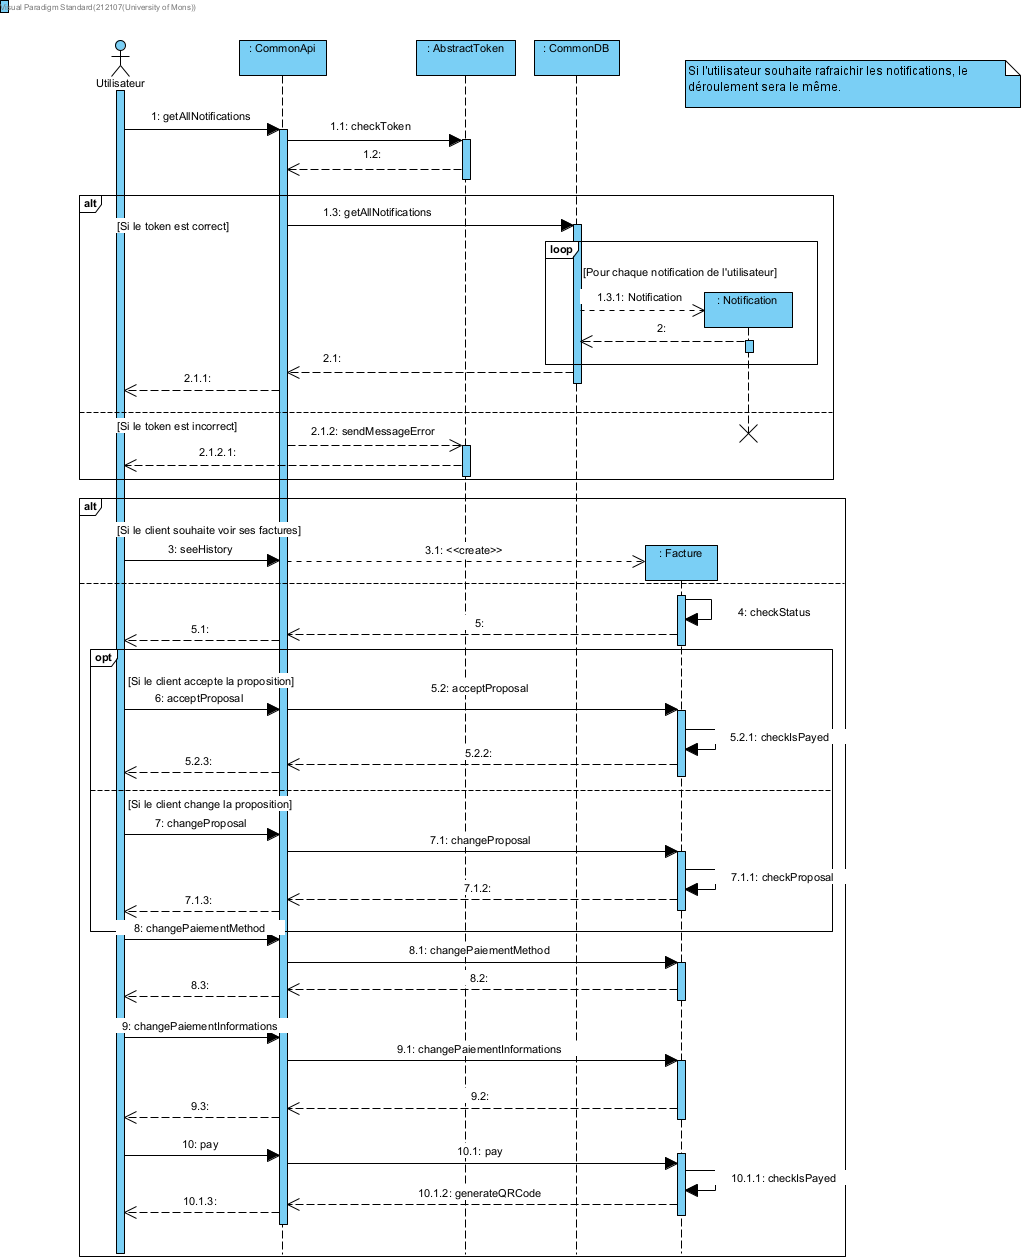
\includegraphics[width = 1]{extension-maxime/sequence/img/sequence-extension.png}
\end{figure}
